\documentclass[a4j,twocolumn,10pt]{jarticle}
\usepackage[dvipdfmx]{graphicx}
\usepackage{url}
\usepackage{color}
\usepackage[dvipdfmx]{hyperref}
\usepackage{pxjahyper}

\title{ミーティング資料}
\author{藤井敦寛}
\date{\today}


\begin{document}
\maketitle

\section{進捗状況}
8Pの校正ですが,全て一度読んだ上で,修正,適用しました.変更点をアップしますので確認お願いします.これ,ISWCで後から変更した部分はまだ加筆してませんが,どうしましょうか.

\section{今週のアイデア}
視線情報を誰もやってないので、その系統をやりたいなと思ってます。
\begin{itemize}
  \item 視線情報からのマイノリティ検出

  カンニングの検知など。

  \item ぼーっとしている状態の検出

  考え事などしていると、眼球運動は一般時に比べて緩やかになる?運転中であれば、注意散漫で警告を出したりできるかもしれない。

  \item 運転中にキョロキョロする回数が少ないと警告

  周囲の確認作業を怠らせない。
\end{itemize}

\section{先週までのキープ案}
\begin{itemize}
  \item 歯ぎしり検知
  \item 起立時の行動特徴からその後の行動推定
  \item 乗り物乗車時の加速度センサのキャリブレーション
  \item 足の筋電から歩幅推定
  \item 歯の裏トラックパッド
\end{itemize}


\section{ボツ案}
\begin{itemize}
  \item 運動強度の可視化
  \item ジョギング時のペース管理
  \item マウスの掌握やキーボードの打鍵の強さ,触れた回数などからコンディションなどの推定
  \item 椅子着座認識
  \item 心電と脈波の時間差から個人識別
  \item 筋電による状態認識
  \item 物理フリックキーボード
  \item プロジェクターのスクリーンをタッチパネル化
  \item 警報音の目的判別
  \item あおり運転に繋がるドライバーの行動変化
  \item ドライバーの疲労度(腕の下がり)
  \item ライダーの疲労度変化(風圧,気温)
  \item グリップ内蔵型スイッチボックス
  \item 次世代型エンジンスタートシステム(ハンドル圧での認証,ドアノブ圧認証)
  \item 次世代型給油停止システム(センサ型)
  \item 人の歩幅を使った何か…疲労度とか?
  \item センサーで眼を観察して動きなどから視力低下限界警告
  \item 1km以上追越車線を走行した場合のアラートと,車線変更可能位置の誘導などの運転支援
  \item 硬筆文字のデジタル化
\end{itemize}

% \begin{figure*}[t]
%   \begin{center}
%     \includegraphics[width=1\textwidth]{Figure_1.eps}
%     \caption{}
%     \label{fig}
%   \end{center}
% \end{figure*}

\end{document}
